\section{Evaluation Framework}

\subsection{Component scores and endpoint targets}
For image $x$ and model $m$, let eligible target component $i$ have coverage
$c_i\in[0,1]$, provenance $p_i\in[0,1]$, and externally assigned severity
$s_i>0$. The candidate score
set includes foreground IoU, Boundary IoU, minimum component coverage,
severity-weighted arithmetic and harmonic means, CVaR quality, false-positive
quality $q_{\mathrm{fp}}=1-r_{\mathrm{fp}}$, and the geometric component
score
\begin{equation}
 q_{\mathrm{comp}} =
 \exp\!\left(\sum_i \frac{s_i^\alpha}{\sum_j s_j^\alpha}
 \log[\epsilon+(1-\epsilon)c_i p_i]\right)
 (1-r_{\mathrm{fp}})^\gamma .
 \label{eq:component-score}
\end{equation}
The implementation sets $\alpha=2$, $\epsilon=10^{-6}$, and $\gamma=1$.
Scores are oriented so that larger values indicate better quality. This score
is one candidate in the comparison, not a universal recommendation.

The declared policy utility is one minus the largest severity-normalized
component risk. Operational utility is the minimum of policy utility and
$q_{\mathrm{fp}}$. An image is labelled as containing a severe miss if an
eligible critical component has coverage below 0.5. A high-false-positive
image has $r_{\mathrm{fp}}\geq0.25$. Their union defines the primary
mixed-failure endpoint. These thresholds and severity weights are experimental
operationalizations, not causal labels of harm or validated deployment costs.

All targets and score components are computed against reference annotations;
these are retrospective, annotation-dependent quality assessments, not
annotation-free online reliability estimates. The false-positive endpoint is
particularly direct: $h_{\mathrm{fp}}=1-r_{\mathrm{fp}}$, so its error score
is $1-h_{\mathrm{fp}}=r_{\mathrm{fp}}$, while its label is
$\mathbb{1}[r_{\mathrm{fp}}\geq0.25]$. Whenever both label classes occur,
this construction yields AUROC 1 by definition. We treat that result as a
check of alignment with a directly constructed endpoint, not as evidence of
general failure-detection ability.

Policy and operational targets are evaluated as rankings of six models within
each image: we compute Spearman rank correlation for each image and average
across images with non-degenerate ranks. Severe-miss, false-positive, and
mixed-failure targets are binary image labels evaluated with AUROC using
$1-h_e$ as the error score. Rank agreement and AUROC therefore estimate
different properties. Neither is a calibration measure, a deployment
threshold, or a guarantee of utility after model selection.

\subsection{Empirical pairwise-conflict bound}
Let $K$ criteria score all $M$ models on image $x$. For model pair
$p=(a,b)$, criterion $k$ gives preference $y_{xpk}\in\{-1,0,+1\}$. After
excluding ties, let $n^+_{xp}$ and $n^-_{xp}$ count preferences in each
direction. Any single ordering must choose one direction for $p$ and thus
disagree with at least $\min(n^+_{xp},n^-_{xp})$ declared preferences. We
aggregate the unavoidable minority count across image--pair instances:
\begin{equation}
 B =
 \frac{\sum_{x,p}\min(n^+_{xp},n^-_{xp})}
      {\sum_{x,p}(n^+_{xp}+n^-_{xp})}.
 \label{eq:bound}
\end{equation}
Criterion ties are defined by exact numerical equality; the implementation
applies no tolerance. The pairwise sum is a lower bound and need not be
attained by a transitive total ordering. Its denominator is the number of
non-tied criterion votes, not the number of images or deployment decisions.
The bound concerns complete strict model rankings. A scalar score that ties
models therefore requires a deterministic tie break; unresolved scalar ties
are not treated as a separate outcome. This is a preference-weighted empirical
lower bound for the finite criterion
set, images, and model panel. It is not the fraction of images with differing
rankings, a fitted-score error, or a theorem about unobserved criteria or
models. The primary estimate excludes ties; sensitivity analyses count ties
as agreement or split them between directions. Confidence intervals resample
images while retaining each image's complete model group, preserving
within-image dependence among model-pair comparisons.

Because a scalar score can realize any strict ordering of the models on an
image, the least disagreement attainable by any scalar is obtained by
enumerating all $M!$ orderings per image. With $M=6$ we enumerate the 720
orderings, count the non-tied criterion votes each one contradicts, take the
per-image minimum, and aggregate as in Eq.~\ref{eq:bound}. We denote the
result $B_{\mathrm{exact}}\geq B$; the gap measures how much intransitivity
across model pairs adds to the pairwise bound.

\paragraph{Social-choice view.} Treating each criterion as a voter that ranks
the models (abstaining on ties), $B_{\mathrm{exact}}$ is the normalized score of
a Kemeny--Young optimal ranking~\cite{kemeny1959mathematics,young1978consistent}:
the least total pairwise disagreement achievable by any strict ranking. $B$ is
the classical pairwise lower bound on that score. It is attained on an image
exactly when some strict ordering agrees with every strict pairwise majority,
so a small gap means majority cycles are rare and the disagreement is pairwise.
Kemeny aggregation is NP-hard in general~\cite{bartholdi1989voting,dwork2001rank},
but exhaustive search is trivial for six models. Arrow's
theorem~\cite{arrow1951social} shows that no rule can aggregate rankings of three
or more alternatives while meeting a small set of natural conditions, but it
does not say how much disagreement any particular aggregate must incur. $B$
and $B_{\mathrm{exact}}$ provide that quantity for the observed preference
profiles: every scalar quality score, being one strict ranking per image, must
contradict at least this share of the declared criteria.

\begin{figure}[t]
  \centering
  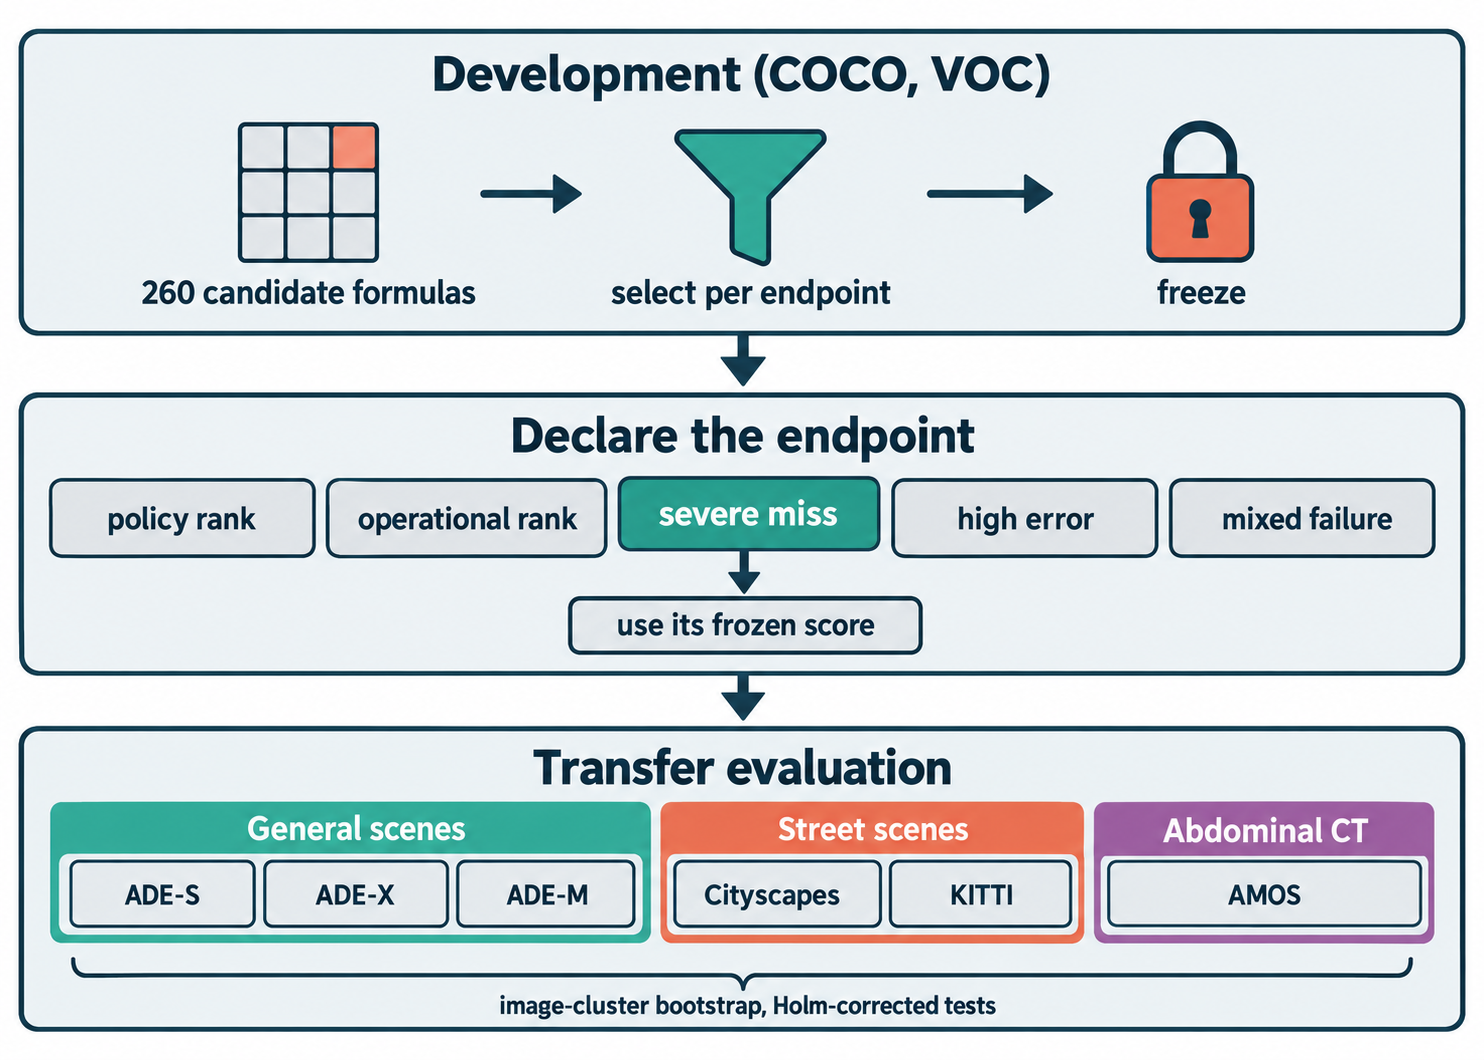
\includegraphics[width=\linewidth]{method_overview.png}
  \caption{Protocol. One score formula per endpoint is selected from 260
  candidates on COCO and VOC and frozen. After an endpoint is declared, its
  frozen score is applied unchanged to the general-scene, street-scene, and CT
  transfer panels, with
  image-cluster bootstrap intervals and Holm-corrected tests.}
  \label{fig:method}
\end{figure}

\subsection{Frozen endpoint-specific scores}
We enumerate single components and convex pairs on a fixed weight grid. The
development selection uses COCO and VOC and requires cross-dataset consensus;
the selected formulas are then frozen:
\begin{align}
 h_{\mathrm{policy}} &= q_{\mathrm{CVaR}}, &
 h_{\mathrm{oper}} &= .1q_{\mathrm{CVaR}}+.9q_{\mathrm{comp}},\\
 h_{\mathrm{severe}} &= .9q_{\mathrm{CVaR}}+.1q_{\mathrm{fp}}, &
 h_{\mathrm{fp}} &= q_{\mathrm{fp}},\\
 h_{\mathrm{mixed}} &= .2q_{\mathrm{comp}}+.8q_{\mathrm{fp}}.
 \label{eq:scores}
\end{align}
For endpoint $e$, routing selects $h_e$ after $e$ has been declared. The
baseline reuses $h_{\mathrm{mixed}}$ for all endpoints. This estimates the
effect of assigning these frozen scores to these declared endpoints; it does
not establish that the formulas outperform every individual metric.

Within-panel comparisons use paired image-cluster bootstrap resampling of
the same image groups: each draw carries all six model records of a sampled
image together. Rank-endpoint draws resample jointly defined image-level
paired differences; AUROC differences are recomputed exactly from the
resampled records in every draw. One-sided empirical $p$-values are
$(1+\#\{\Delta^*\leq0\})/(B+1)$ from 5,000 draws. The \NFamilyN{}
panel-by-endpoint tests (eight panels by five endpoints) are Holm-adjusted
together at $\alpha=0.05$, including the eight mixed-failure identity
comparisons. Intervals are conditional on the six observed checkpoints and
fixed endpoint definitions; they do not quantify variation over future
datasets or architectures. Aggregates across panels are descriptive, because
panels are not independent draws from a defined population and the three
ADE20K panels share images.

\subsection{Domain-matched failure score}
A failure score selected on one domain may not suit another whose failures
differ in kind. To test whether matching the selection data to the target
domain helps, we re-run the 260-formula selection for the mixed-failure
endpoint on Cityscapes training records only (\NSelDevRecords{} model--image
records, of which \NSelDevSevere{} are severe misses and \NSelDevHigh{} are
high-error failures), freeze the selected formula, and compare it with the
general-scene mixed score on three held-out panels: Cityscapes validation,
KITTI, and AMOS CT. Differences use the exact cluster bootstrap above with Holm
correction over the three panels.
